\documentclass[border=3pt]{standalone}
% Preâmbulo compartilhado pelos diagramas TikZ da aula
\usepackage[T1]{fontenc}
\usepackage[utf8]{inputenc}
\usepackage{lmodern}
\usepackage{amsmath}
\usepackage{xcolor}
\usepackage{tikz}
\usetikzlibrary{arrows.meta,angles,quotes,decorations.pathmorphing,calc,
                positioning,shapes.geometric,backgrounds,fit}

% Paleta (mesma dos SVGs originais)
\definecolor{dblue}{HTML}{2A5B8C}
\definecolor{dorange}{HTML}{B3541E}
\definecolor{dgreen}{HTML}{4A7C59}
\definecolor{dred}{HTML}{9C4B4B}
\definecolor{dcream}{HTML}{F4F1EA}
\definecolor{dshade}{HTML}{DDD7C9}

% Estilos comuns (prefixo d... para não colidir com chaves internas do pgf)
\tikzset{
  >={Stealth[length=2mm]},
  dguide/.style={gray!55, dashed, line width=0.4pt},
  daxis/.style={gray!60, line width=0.7pt, ->},
  dbody/.style={fill=black!3, draw=black!80, line width=1pt},
  dacc/.style={draw=dblue, line width=1pt},
  dlbl/.style={black!55, font=\small},
  dsub/.style={black!45, font=\footnotesize},
  dstate/.style={circle, draw=black!80, fill=dcream, line width=1pt,
                 minimum size=17mm, font=\large, inner sep=1pt},
  dobs/.style={circle, draw=black!80, fill=dshade, line width=1pt,
               minimum size=14mm, font=\large, inner sep=1pt},
  dbox/.style={rounded corners=2pt, draw=black!80, fill=dcream, line width=1pt,
               align=center, inner sep=6pt},
  dtrans/.style={->, dblue, line width=1pt},
  dmeas/.style={->, dorange, line width=1pt},
}

\begin{document}
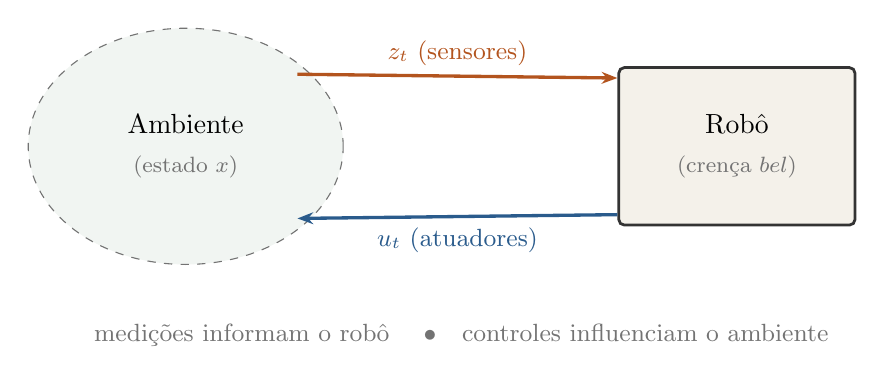
\begin{tikzpicture}[x=1cm,y=1cm]

  % ambiente
  \node[draw=black!55, dashed, ellipse, minimum width=4cm, minimum height=3cm,
        fill=dgreen!8, align=center] (env) at (0,0)
        {\normalsize Ambiente\\[2pt]\footnotesize\textcolor{black!55}{(estado $x$)}};

  % robô
  \node[dbox, minimum width=3cm, minimum height=2cm] (rob) at (7,0)
        {\normalsize Robô\\[2pt]\footnotesize\textcolor{black!55}{(crença $bel$)}};

  % medição: ambiente -> robô
  \draw[dmeas, line width=1.2pt] (env.north east) ++(0,-0.15)
        -- node[above, dorange, font=\small] {$z_t$ (sensores)}
           ($(rob.north west)+(0,-0.15)$);

  % controle: robô -> ambiente
  \draw[dtrans, line width=1.2pt] ($(rob.south west)+(0,0.15)$)
        -- node[below, dblue, font=\small] {$u_t$ (atuadores)}
           ($(env.south east)+(0,0.15)$);

  \node[dlbl] at (3.5,-2.4)
    {medições informam o robô \quad$\bullet$\quad controles influenciam o ambiente};

\end{tikzpicture}
\end{document}
